\section{Results}
In the following section we will present our results, and numerical considerations, relevant for overviewing the possible consequences of NCG at modern collider experiments. We will give an estimate on the possible scale of a NCG theory, and what impact this will have on cross sections for processes involving the $Z$ boson.

\subsection{Setting constraints on $\Lambda$ using LEP data}
To set a constraint on the possible values of $\theta = \frac{1}{\Lambda^2}$ we can look at the width of $\Gamma_{Z \rightarrow gg}$ as predicted by NCG. Now, we have not seen effects of NCG greater than the uncertainty in current experimental data, additional contribution to the total $Z^0$ width, coming from $Z \rightarrow gg$ processes, must thus be lower than the current uncertainty $\Gamma_{Z \rightarrow gg} < 1 \times 10^{-3}$ GeV \cite{behr2003dnc}. To see how this puts a constraint on $\theta$ we use an expression for $\Gamma_{Z \rightarrow gg}$ taken from \cite{behr2003dnc};
\begin{equation} \label{eq:zggwidth}
	\Gamma_{Z \rightarrow gg} = \frac{8}{12} K_{gg}^2 \alpha M_Z^5 \sin^22\theta_W \frac{1}{\Lambda^4}.
\end{equation}
In figure \ref{fig:kplot} we have made a plot of the minimum allowed value for $\Lambda$. Allowed values of $K_{gg}$ lies in the interval $\{-0.1,0.2\}$ \cite{behr2003dnc}, so our maximum lower bound for $\Lambda$ is found for $K_{gg}=0.2$. This gives the experimental minimal value $\Lambda >132$ GeV.
\includefigure{fig:kplot}{0.3}{./images/kplot}{Plot of the allowed region for $\Lambda$ and $K_{gg}$. The filled area represent the constraint $\Gamma_{Z \rightarrow gg} < 0.001 \textrm{ GeV}$ as set by equation \eqref{eq:zggwidth}. Allowed $K_{gg}$ is in the region $\{-0.1,0.2\}$ represented by the black box in the figure.}

\subsection{Cross sections for different $\Lambda$ compared to SM}
Below we have drawn histograms showing the expected number of event at LHC (with $L=10 \textrm{ fb}^{-1}$) from colliding protons, producing muon-pairs through leading order diagrams (Figures \ref{fig:feyn:parton_qq} and \ref{fig:feyn:parton_gg}) of the process $pp \rightarrow Z \rightarrow \mu \bar \mu$, together with the contribution as predicted by NCG. All interference terms have been ignored. As have contributions from diagrams involving vertices $\gamma gg$. Four different plots are made for different values of $\Lambda$. The statistical error, $1/\sqrt{N}$, where $N$ is the number of events in the given bin, for standard events are shown by the gray band.

\begin{figure}[htp]
	\centering
	\begin{minipage}[b]{0.475\linewidth} 
    \centering
	  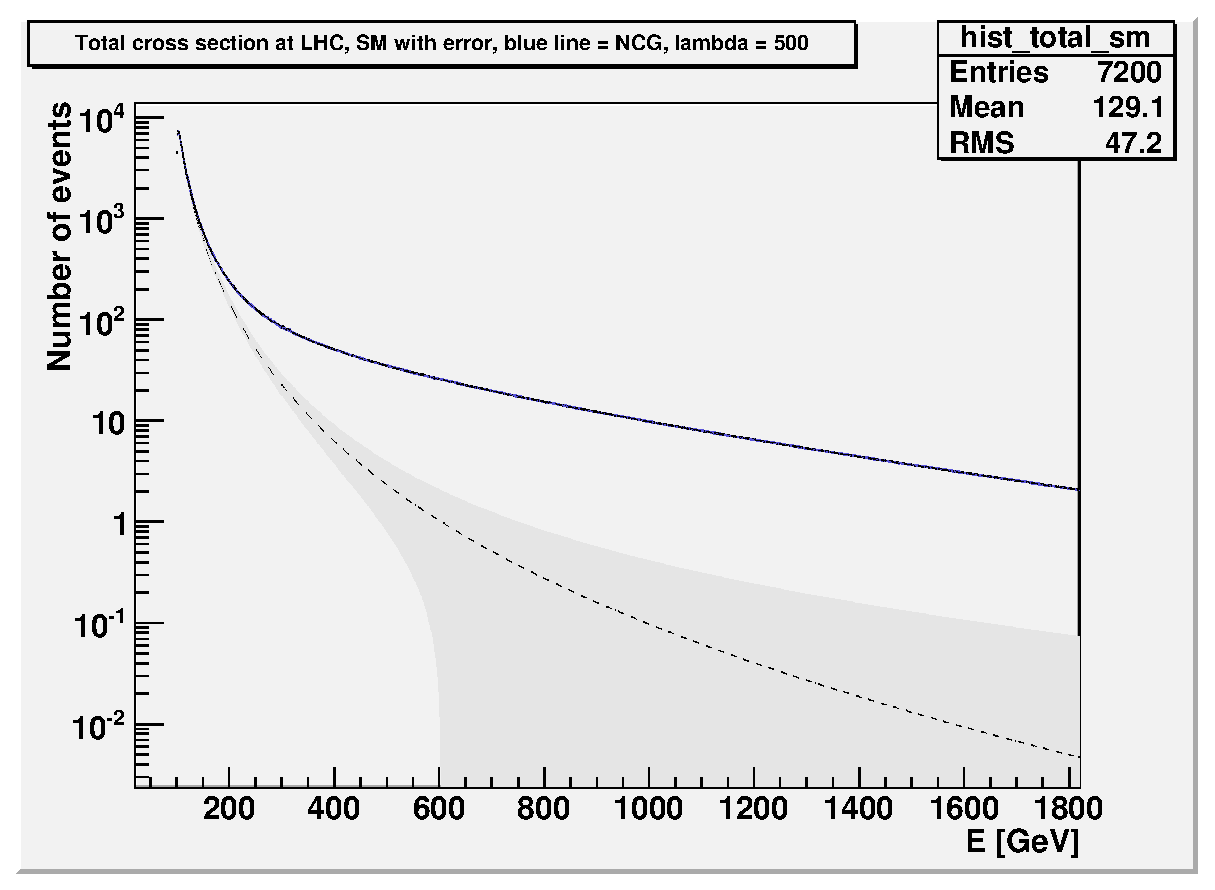
\includegraphics[scale=0.35]{./images/L500r139.eps}
	\end{minipage}
	\hspace{0.5cm}
	\begin{minipage}[b]{0.475\linewidth} 
    \centering
	  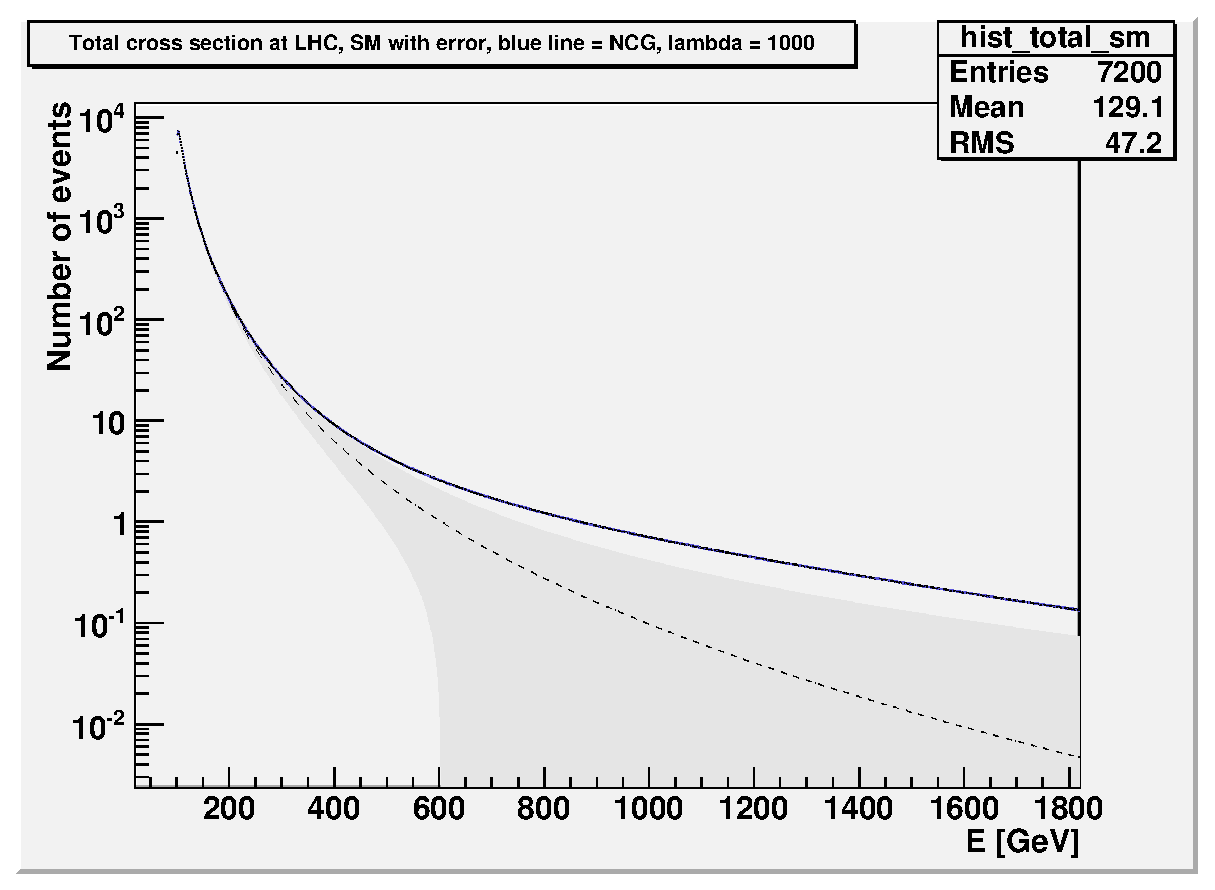
\includegraphics[scale=0.35]{./images/L1000r139.eps}
	\end{minipage}
	\\ \vspace{0.5cm}
	\begin{minipage}[b]{0.475\linewidth} 
    \centering
	  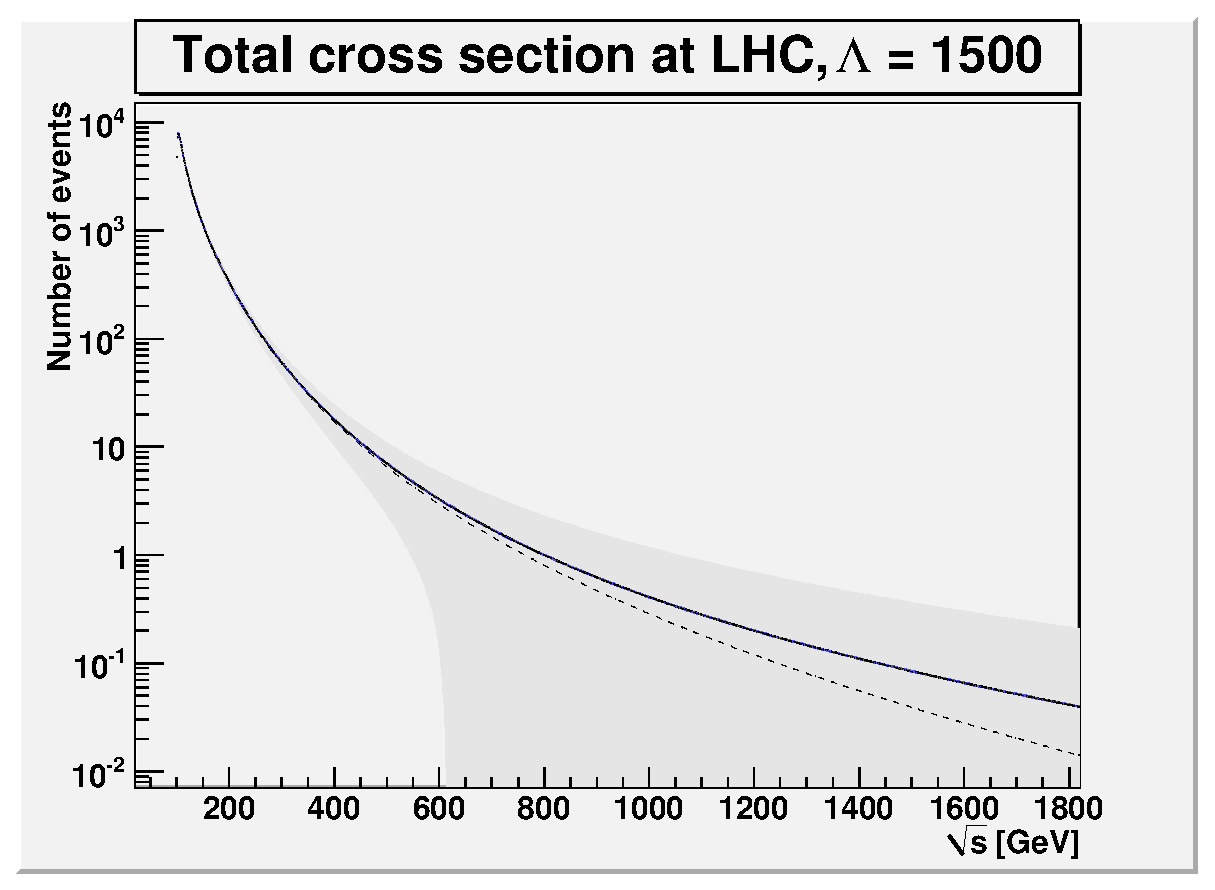
\includegraphics[scale=0.35]{./images/L1500r139.eps}
	\end{minipage}
	\hspace{0.5cm}
	\begin{minipage}[b]{0.475\linewidth} 
    \centering
	  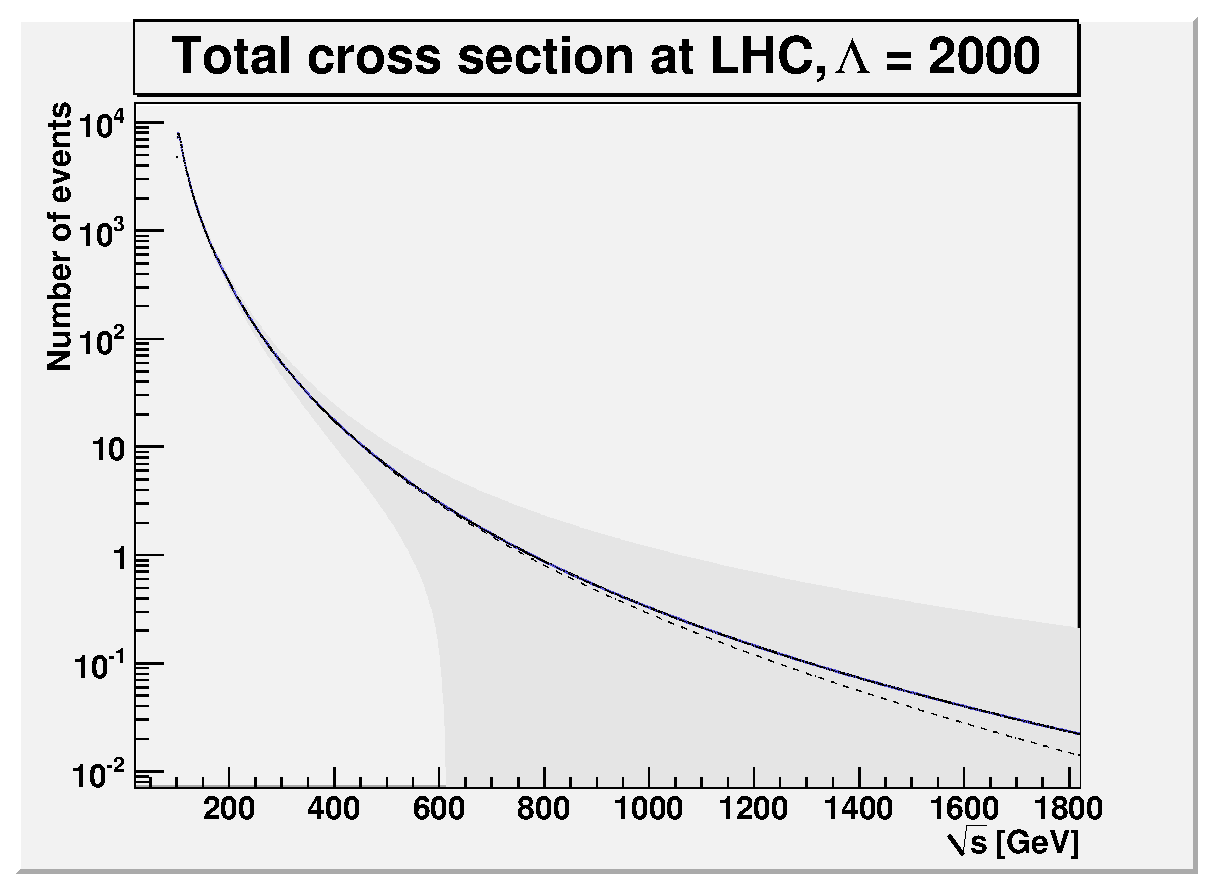
\includegraphics[scale=0.35]{./images/L2000r139.eps}
	\end{minipage}
		\caption{Predicted number of $pp \rightarrow Z/ \gamma \rightarrow \mu \bar \mu$ events at LHC running with a luminosity of $L=10 \textrm{ fb}^{-1}$ for one year. The grey line shows number of events as predicted by the SM with error of $1/\sqrt{N}$, where $N$ is the number of events in the given bin. The blue line represent number of events as predicted by NCG for the given value of $\Lambda$. All interference terms and possible NCG contributions from $\gamma gg$ vertices have been ignored.}
\end{figure}